\documentclass{beamer}
\mode<presentation>
\usepackage{amsmath}
\usepackage{amssymb}
%\usepackage{advdate}
\usepackage{adjustbox}
\usepackage{subcaption}
\usepackage{enumitem}
\usepackage{multicol}
\usepackage{mathtools}
\usepackage{listings}
\usepackage{url}
\def\UrlBreaks{\do\/\do-}
\usetheme{Boadilla}
\usecolortheme{lily}
\setbeamertemplate{footline}{
  \leavevmode%
  \hbox{%
    \begin{beamercolorbox}[wd=.9\paperwidth,ht=2.25ex,dp=1ex,left]{author in head/foot}%
      \hspace{1em} Balaji B % Your name here
    \end{beamercolorbox}%
    \begin{beamercolorbox}[wd=.1\paperwidth,ht=2.25ex,dp=1ex,right]{author in head/foot}%
      \insertframenumber{} / \inserttotalframenumber\hspace*{2ex}
    \end{beamercolorbox}}%
}
\setbeamertemplate{navigation symbols}{}

\providecommand{\nCr}[2]{\,^{#1}C_{#2}} % nCr
\providecommand{\nPr}[2]{\,^{#1}P_{#2}} % nPr
\providecommand{\mbf}{\mathbf}
\providecommand{\pr}[1]{\ensuremath{\Pr\left(#1\right)}}
\providecommand{\qfunc}[1]{\ensuremath{Q\left(#1\right)}}
\providecommand{\sbrak}[1]{\ensuremath{{}\left[#1\right]}}
\providecommand{\lsbrak}[1]{\ensuremath{{}\left[#1\right.}}
\providecommand{\rsbrak}[1]{\ensuremath{{}\left.#1\right]}}
\providecommand{\brak}[1]{\ensuremath{\left(#1\right)}}
\providecommand{\lbrak}[1]{\ensuremath{\left(#1\right.}}
\providecommand{\rbrak}[1]{\ensuremath{\left.#1\right)}}
\providecommand{\cbrak}[1]{\ensuremath{\left\{#1\right\}}}
\providecommand{\lcbrak}[1]{\ensuremath{\left\{#1\right.}}
\providecommand{\rcbrak}[1]{\ensuremath{\left.#1\right\}}}
\theoremstyle{remark}
\newtheorem{rem}{Remark}
\newcommand{\sgn}{\mathop{\mathrm{sgn}}}
\providecommand{\abs}[1]{$\left \vert#1\right\vert$}
\providecommand{\res}[1]{\Res\displaylimits_{#1}} 
\providecommand{\norm}[1]{\lVert#1\rVert}
\providecommand{\mtx}[1]{\mathbf{#1}}
\providecommand{\mean}[1]{E$\left[ #1 \right ]$}
\providecommand{\fourier}{\overset{\mathcal{F}}{ \rightleftharpoons}}
%\providecommand{\hilbert}{\overset{\mathcal{H}}{ \rightleftharpoons}}
\providecommand{\system}{\overset{\mathcal{H}}{ \longleftrightarrow}}
	%\newcommand{\solution}[2]{\textbf{Solution:}{#1}}
%\newcommand{\solution}{\noindent \textbf{Solution: }}
\providecommand{\dec}[2]{\ensuremath{\overset{#1}{\underset{#2}{\gtrless}}}}
\newcommand{\myvec}[1]{\ensuremath{\begin{pmatrix}#1\end{pmatrix}}}
\let\vec\mathbf

\lstset{
%language=C,
frame=single, 
breaklines=true,
columns=fullflexible
}

\numberwithin{equation}{section}
\title{12.8.2.6}
\author{Balaji Balamurugan \\ Dept. of Electrical Engineering \\ IIT Hyderabad}

\date{\today} 

\begin{document}

\begin{frame}
\titlepage
\end{frame}

\section*{Outline}
\begin{frame}
\tableofcontents
\end{frame}

\section{Question}
\begin{frame}
\frametitle{Question}
Smaller area enclosed by the circle $x^2 + y^2 = 4 $ and the line $x + y = 2 $ is 
\end{frame}

\section{Solution}
\subsection{Parameters}
\begin{frame}
\frametitle{Parameters}
The parameters for the problem are given as follows:
\begin{table}[H]
    \centering
    \begin{tabular}[12pt]{ |c| c| c |}
    \hline
    \textbf{Variable} & \textbf{Description} & \textbf{values}\\ 
    \hline
    $\vec{V}$ & Quadratic form of the matrix & $\myvec{1 & 0 \\ 0 & 1} $\\
    \hline
    $\vec{u}$ & Linear coefficient vector & $\myvec{0 \\ 0} $\\
    \hline
    f & constant term & -4 \\ 
    \hline
    $\vec{m}$ & The direction vector of line & $\myvec{1 \\ -1}$\\
    \hline
     $\vec{h}$ & Point on line & \myvec{2 \\ 0} \\
     \hline
\end{tabular}
    \caption{Parameter Used}
    \label{tab1-1.9-6}
\end{table}

\end{frame}

\subsection{Theoretical Solution}
\begin{frame}
\frametitle{Theoretical Solution}

The point of intersection of the line with the circle is $x_i=h+k_i m$,\\
where, $k_i$ is a constant and is calculated as follows:-
$$k_i=\frac{1}{m^\top Vm}\brak{-m^\top \brak{Vh+u}\pm \sqrt{\sbrak{m^\top \brak{Vh+u}}^ 2-g\brak{h}\brak{m^\top Vm}}}$$\\
Substituting the input parameters into $k_i$,\\
{\scriptsize
\begin{multline}
     k_i =\frac{1}{\myvec{1 
 & -1}\myvec{1 & 0 \\ 0 & 1}\myvec{1 \\ -1}}\brak{-\myvec{1&-1}\brak{\myvec{1&0\\0&1}\myvec{2\\0}+\myvec{0\\0}}}\pm \\
     \sqrt{\sbrak{\myvec{1&-1}\brak{\myvec{1&0\\0&1}\myvec{2\\0}+\myvec{0\\0}}}^2-g\brak{h}\brak{\myvec{1&-1}\myvec{1&0\\0&1}\myvec{1\\-1}}} 
\end{multline}
}
\end{frame}
\begin{frame}
We get,\\
$k_i= 0,-2$\\
Substituting $k_i$ into $x_i=h+k_i m$ we get\\
    For the given line $x=4a$, The values of $\vec{h}$, $\vec{m}$ are
\begin{align}
     x_1&=\myvec{2\\0}+\brak{0}\myvec{1\\-1}\\
    \implies x_1 &=\myvec{2\\0}\\
    x_2 &=\myvec{2\\0}+\brak{-2}\myvec{1\\-1}\\
    \implies x_2&=\myvec{2\\0}+\myvec{-2\\2}\\
    \implies x_2&=\myvec{0\\2}
\end{align}
\end{frame}
\begin{frame}
    The area of the smaller region bounded by the circle $x^2 + y^2 = 4$ and the line $x + y = 2$ is
\begin{align}
    &=\int_{0}^{2} \sqrt{4-x^2}dx-\int_{0}^{2} \brak{2-x} dx\\
    &=\brak{\frac{x}{2}\sqrt{4-x^2}+\frac{4}{2}\sin^{-1}{\frac{x}{2}}-2x+\frac{x^2}{2}}_{0}^{2}\\
    &=\brak{\pi-2}
\end{align}
\end{frame}
\subsection{Computational Solution}
\begin{frame}
\frametitle{Computational Solution}
Taking trapezoid-shaped strips of small area and adding them all up. Say we have to find the area of $y_{x}$ from $x=x_0$ to $x=x_n$, discretize the points on the $x$ axis $x_0, x_1, x_2, \dots, x_n$ such that they are equally spaced with the step size $h$. \\
Sum of all trapezoidal areas is given by,
{\small
\begin{align}
  A&=\frac{1}{2}h\brak{y\brak{x_1}+y\brak{x_0}}+ \frac{1}{2}h\brak{y\brak{x_2}+y\brak{x_1}}+\dots+\frac{1}{2}h\brak{y\brak{x_n}+y\brak{x_{n-1}}}\\
  &=h\sbrak{\frac{1}{2}\brak{y\brak{x_0}+y\brak{x_n}}+ y\brak{x_1}+\dots+y\brak{x_{n-1}}}
\end{align}
}
Let $A\brak{x_n}$ be the area enclosed by the curve $y\brak{x}$ from $x=x_0$ to $x=x_n$, $\brak{x_0, x_1, \dots x_n}$ be equidistant points with step-size $h$.
\begin{align}
  A\brak{x_n+h}=A\brak{x_n}+\frac{1}{2}h\brak{y\brak{x_n+h}+y\brak{x_n}}
\end{align}
\end{frame}
\begin{frame}
We can repeat this till we get required area.\\
Discretizing the steps, making $A\brak{x_n}=A_n, y\brak{x_n}=y_n$ we get,
\begin{align}
 A_{n+1}=A_n+\frac{1}{2}h\brak{y_{n+1}+y_n}
\end{align}
We can write $y_{n+1}$ in terms of $y_n$ using first principle of derivative. $y_{n+1}=y_n+hy^{\prime}_n$
\begin{align}
  A_{n+1}&=A_n+\frac{1}{2}h\brak{\brak{y_{n}+hy^{\prime}_n}+y_n}\\
  A_{n+1}&=A_n+\frac{1}{2}h\brak{2y_n+hy^{\prime}_n}\\
  A_{n+1}&=A_n+hy_n+\frac{1}{2}h^2y^{\prime}_n\\
  x_{n+1}&=x_n+h
\end{align}
\end{frame}
\begin{frame}
    In the given question, $y_n=\sqrt{4-x_n^2} + x_n -2$ and $y^{\prime}_n= \frac{-x_n}{\brak{\sqrt{4-x_n^2}}} +1 $\\
The general difference equation will be given by
\begin{align}
  A_{n+1}&=A_n+hy_n+\frac{1}{2}h^2y^{\prime}_n\\
  A_{n+1}&=A_n+h\brak{\sqrt{4-x_n^2} + x_n -2}+\frac{1}{2}h^2\brak{\frac{-x_n}{\brak{\sqrt{4-x_n^2}}} +1}\\
  x_{n+1}&=x_n+h
\end{align}
Iterating till we reach $x_n=2$ will return required area. \\
Area obtained computationally: $1.41555$ sq. units\\
Area obtained theoretically: $\brak{\pi - 2}$ sq. units = 1.14 sq.unis
\end{frame}

\subsection{Plot}
\begin{frame}
\frametitle{Plot}
\begin{figure}[h!]
   \centering
   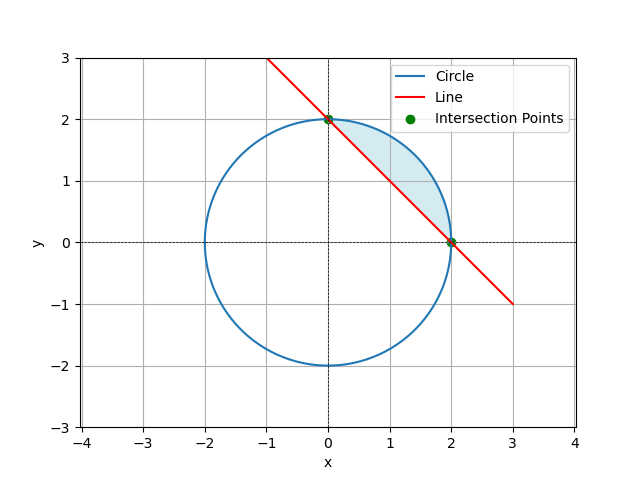
\includegraphics[width=1\columnwidth]{figs/fig.png}
   \caption{Graph of the circle $x^2 + y^2 = 4$ and $x + y = 2 $ and the area enclosed between them}
   \label{stemplot}
\end{figure}
\end{frame}
\begin{frame}{Codes}
   Code: https://github.com/Balaji29-code/EE1003/tree/main/Problem-2/codes
\end{frame}





\end{document}


